\section{Results}

\begin{figure}[ht]
    \centering
    \includegraphics[width=0.45\textwidth]{figures/dist_fig_hist.png}
    \caption{Relative error for the pairwise-distances of CNT, CN3, and ZCNT methods on simulated data as described in Section~\ref{section:comp_dist}. This includes error from multiple test suites where the number of cells was 200 and the loci were from \{1000, 2000, 3000, 4000\}. The graph was then normalized so that the area under the curve for each comparision class would equal 1.}\label{fig:dist_figure_histogram}
\end{figure}

\begin{figure}[ht]
    \centering
    \includegraphics[width=0.45\textwidth]{figures/dist_fig_boxplot.png}
    \caption{Relative error for the pairwise-distances of CNT, CN3, and ZCNT methods on simulated data as described in Section~\ref{section:comp_dist}. Note that outliers are removed int this plot. This includes error from multiple test suites where the number of cells was 200 and the loci were from \{1000, 2000, 3000, 4000\}. The graph was then normalized so that the area under the curve for each comparision class would equal 1.}\label{fig:dist_fig_box}
\end{figure}

\begin{figure}[ht]
    \centering 
    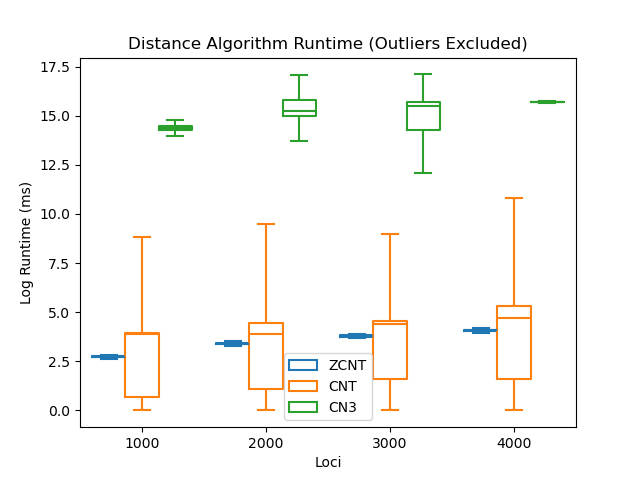
\includegraphics[width=0.45\textwidth]{figures/time_fig.png}
    \caption{This shows the running times of running the different distance methods on different numbers of loci on a logorithmic scale. All trials used 200 cells. This was computed using simulated data. The number of loci were from \{1000, 2000, 3000, 4000\}.}\label{fig:time_fig}
\end{figure} 

The results for the methods described in Section~\ref{section:comp_dist} to compare the three distance algorithms ZCNT, CNT, and CN3 are shown in Figures~\ref{fig:dist_figure_histogram} and~\ref{fig:dist_fig_box} include five suites with a constant number of 200 cells. This data was plotted into a histogram included as Figure~\ref{fig:dist_figure_histogram}. More data was not acquired due to the running time involved in calculating CN3 distances. A figure demonstrating this running time is included as Figure~\ref{fig:time_fig}.

Figures~\ref{fig:dist_figure_histogram} and~\ref{fig:dist_fig_box} show that ZCNT and CN3 have more in common than any other pairing. However the relative error for the grand majority of the comparision classes falls below $10\%$. Interestingly, even the most different pairing (ZCNT and CNT) mostly had error falling below $20\%$. These results do not include pairs with infinite CNT values as those are considered when we do analysis on the absolute values of distances across classes (Figure~\ref{fig:classes_hist}). 

\begin{figure}[ht]
    \centering
    \includegraphics[width=0.45\textwidth]{figures/classes_hist.png}
    \caption{Absolute value of pairwise distances generated with ZCNT according to Section~\ref{section:behavior}. Class 1 is composed of ZCNT distances $\zcnt(u, v)$ where $\cnt(u, v) \neq \infty$ and $\cnt(v, u) \neq \infty$. Class 2 is composed of ZCNT distances $\zcnt(u, v)$ where $\cnt(u, v) \neq \infty$ and $\cnt(v, u) = \infty$. Class 3 is composed of ZCNT distances where $\cnt(u, v) = \cnt(v, u) = \infty$. The distances are from simulated data where the number of cells were in \{200 300 400 500 600 1200\} and the number of loci were from \{1000, 2000, 3000, 4000\} across seven random seeds. The data was then binned and normalized so the area under each curve is 1.}\label{fig:classes_hist}
\end{figure}

\begin{figure}[ht]
    \centering
    \includegraphics[width=0.45\textwidth]{figures/classes_box.png}
    \caption{Absolute value of pairwise distances generated with ZCNT according to Section~\ref{section:behavior}. Class 1 is composed of ZCNT distances $\zcnt(u, v)$ where $\cnt(u, v) \neq \infty$ and $\cnt(v, u) \neq \infty$. Class 2 is composed of ZCNT distances $\zcnt(u, v)$ where $\cnt(u, v) \neq \infty$ and $\cnt(v, u) = \infty$. Class 3 is composed of ZCNT distances where $\cnt(u, v) = \cnt(v, u) = \infty$. The distances are from simulated data where the number of cells were in \{200 300 400 500 600 1200\} and the number of loci were from \{1000, 2000, 3000, 4000\} across seven random seeds. The data was then binned and normalized so the area under each curve is 1.}\label{fig:classes_box}
\end{figure}

Figures~\ref{fig:classes_hist} and~\ref{fig:classes_box} shows the results from the methodology described in Section~\ref{section:behavior}. The three classes seem to all follow fairly normal distributions. Class 1 has the lowest mean while class 3 has the highest mean. This seems to signify to me that reachability in CNT corresponds to lower ZCNT values. This is good because if trees minimize distance, they will also likely favor pairings that are biologically feasible. 


Figures~\ref{fig:illegal_desc} and~\ref{fig:illegal_edges} show the results from the methodology described in Section~\ref{section:simulated_reachability}. These show that as the number of loci increases, biologically infeasible edges become less common. The number of cells involved in the phylogeny appears to decrease the spread of the data, but not shift it. It also shows that biologically infeasible edges are relatively rare, with 22 out of 168 trees (13.09\%) having no illegal edges or ancestor-descendant relationships. The rate of illegal edges is very infrequent with is very small. Even the tree with the most illegal edges has at most 7.36\% of illegal edges. 

\begin{figure}[ht]
    \centering
    \includegraphics[width=0.45\textwidth]{figures/illegal_desc.png} 
    \caption{The percentage of overall ancestor-descendant pairs in Lazac-produced trees on simulated data where it would be biologically infeasible for the descendant to be produced from the ancestor. The number of cells were in \{200 300 400 500 600 1200\} and the number of loci were from \{1000, 2000, 3000, 4000\} across seven random seeds.}
\end{figure}\label{fig:illegal_desc}

\begin{figure}[ht]
    \centering
    \includegraphics[width=0.45\textwidth]{figures/illegal_edges.png}
    \caption{The percentage of overall edges in Lazac-produced trees on simulated data where it would be biologically infeasible for the child to be produced from the parent. The number of cells were in \{200 300 400 500 600 1200\} and the number of loci were from \{1000, 2000, 3000, 4000\} across seven random seeds.}\label{fig:illegal_edges}
\end{figure}

\begin{figure}[ht]
    \centering
    \includegraphics[width=0.45\textwidth]{figures/cumulative_plot.png}
    \caption{This shows a cumulative plot that shows what percentage of simulated trees contain biologically infeasible edges or ancestor-descendent relationships. The number of cells were in \{200 300 400 500 600 1200\} and the number of loci were from \{1000, 2000, 3000, 4000\} across seven random seeds.}\label{fig:cumulative_trees}
\end{figure}

Figure~\ref{fig:cumulative_trees} shows the cumulative rate of illegal edges or ancestor-descendant relationships. Illegal edges are the source of illegal ancestor-descendant relationships so the ancestor-descendant curve is just a horizontally stretched version of the illegal edges curve. The amount of stretch shows how many cells are descended from illegal edges. 

The plot shows that more than half the trees have fewer than 2.5\% illegal edges. The trees with the fewest illegal edges don't appear to have many descendants of those illegal relationships as shown by the curves matching for the first portion of the graph. This implies that for those trees, the ZCNT model predicts very biologically feasible trees. However for roughly 40\% of the trees, an increasing proportion of nodes are descended from improssible transitions like zero-amplifications. 